\documentclass[border=0.8ex,svgnames,tikz]{standalone}
\usepackage{amsmath,mathtools}
\usepackage{fontspec}
\setmainfont{Source Serif 4}
\setsansfont{Source Sans 3}
\setmonofont{Source Code Pro}
\usetikzlibrary{shapes.multipart}
\begin{document}
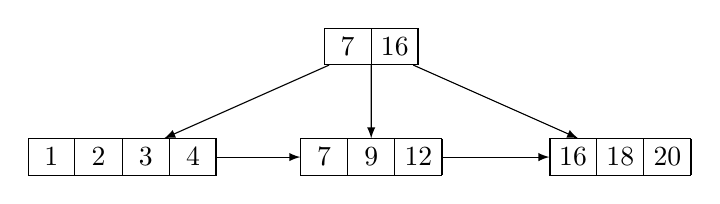
\begin{tikzpicture}[
  level distance=4em,
  every node/.style={
    draw,
    align=center,
    rectangle split,
    rectangle split horizontal,
    rectangle split ignore empty parts,
  },
  level 1/.style={sibling distance=9em},
  every one node part/.style={text width=1em},
  every two node part/.style={text width=1em},
  every three node part/.style={text width=1em},
  every four node part/.style={text width=1em},
  every path/.style={draw,>=latex},
  ]
  \node(n0){\nodepart{one}7 \nodepart{two}16}
  [->]
  child{
    node(n1){\nodepart{one}1 \nodepart{two}2 \nodepart{three}3 \nodepart{four}4}
  }
  child{
    node(n2){\nodepart{one}7 \nodepart{two}9 \nodepart{three}12}
  }
  child{
    node(n3){\nodepart{one}16 \nodepart{two}18 \nodepart{three}20}
  };
  \path[->]
  (n1) edge (n2)
  (n2) edge (n3);
\end{tikzpicture}
\end{document}
